%
% tests
% @author Tobias Weber <tweber@ill.fr>
% @date aug-2021
% @license see 'LICENSE' file
%

\chapter{Test Tools and Unit Tests}
\label{ch:tests}
Due to a rapid increase in complexity over time, the software of this work 
necessitated a multi-tiered testing strategy during development.
But also after having finished the critical phases of development, the test tools presented in this 
chapter serve to ensure that the software and its parts continue to work as intended. 
Problems that may arise can be rapidly analysed using the simplified environments these tools provide.

Before being integrated into the main library or the GUI program, each essential function was tested 
separately. Either via small test programs or via dedicated unit tests, which are discussed in 
section \ref{sec:unit_tests}.
Integration tests of algorithms and collections of functions were performed using larger test programs 
which implemented a simplified versions of the functionality of the main programs.
These are described in section \ref{sec:tests_tools}.



\section{Test tools}
\label{sec:tests_tools}


\subsection{Line segments tool}
\begin{figure}[htb]
	\centering
	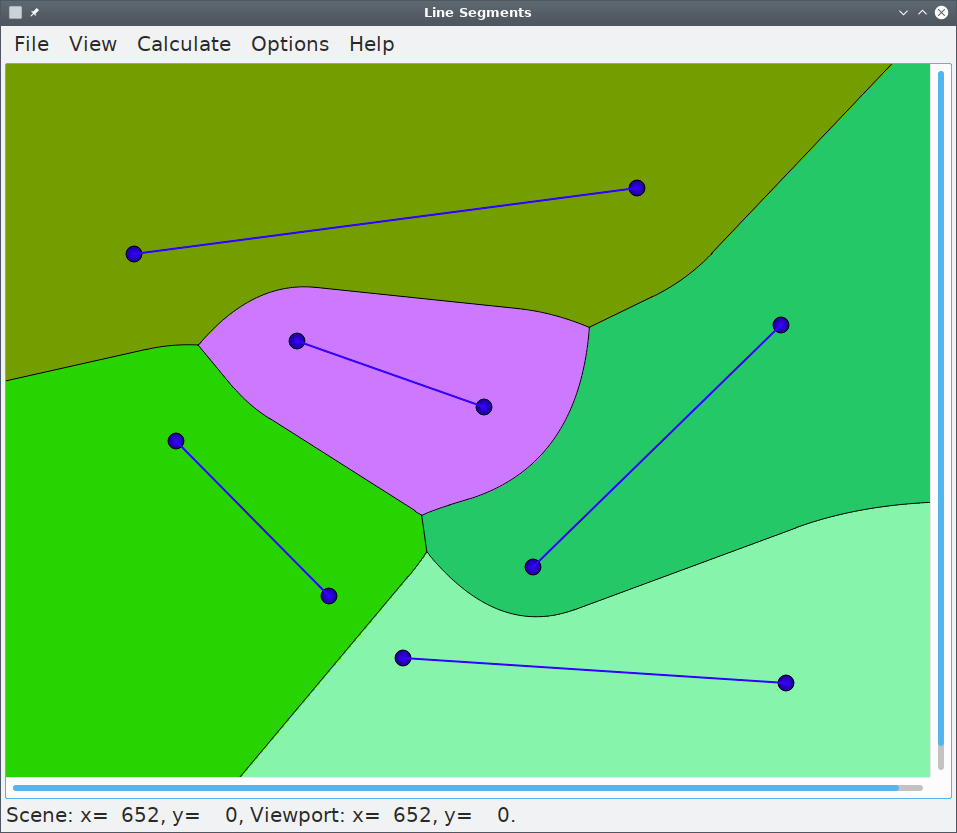
\includegraphics[width = 0.49 \textwidth]{figures/linesgui_voro}
	\hspace{0.05cm}
	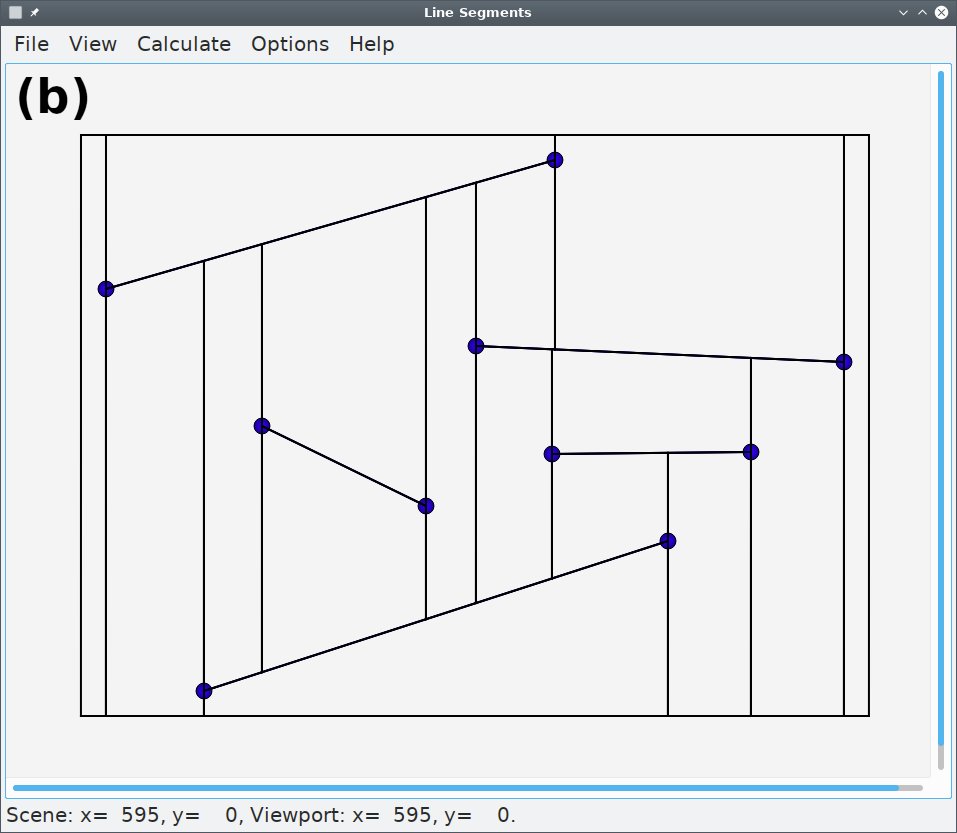
\includegraphics[width = 0.49 \textwidth]{figures/linesgui_trapezoid}

	\vspace{0.25cm}
	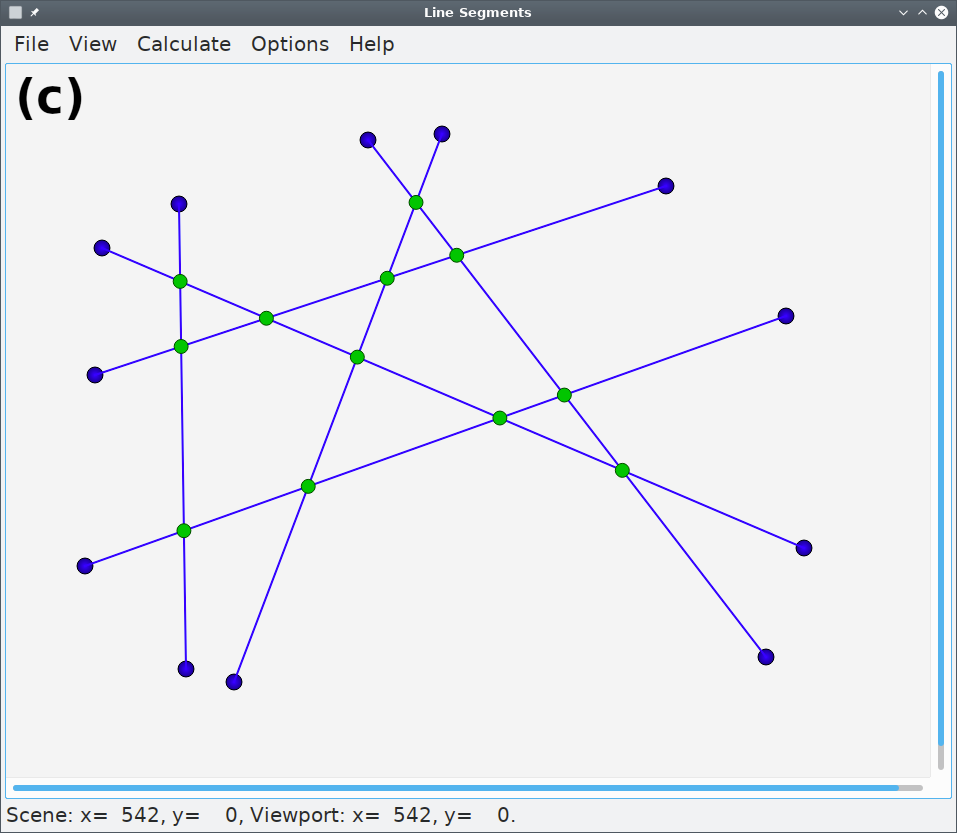
\includegraphics[width = 0.49 \textwidth]{figures/linesgui_inters}
	\caption[Line segments tool.]{Line segments tool.
		This program allows the dynamic calculation of
		(a) line segment Voronoi regions (coloured) and bisectors (black lines),
		(b) trapezoid maps, and
		(c) sweep-based points of intersection (green points).
		Line segment vertices can be inserted, deleted and moved using the mouse.
		\label{fig:linesgui}}
\end{figure}



\subsection{Polygon tool}
\begin{figure}[htb]
	\centering
	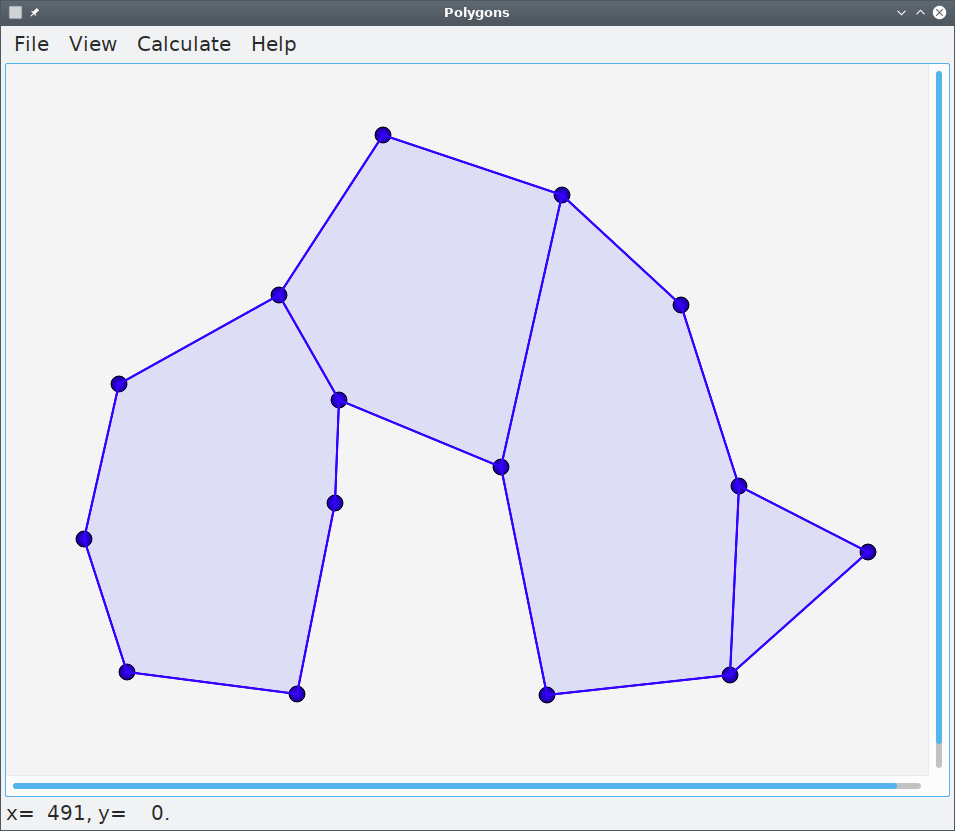
\includegraphics[width = 0.49 \textwidth]{figures/polygui_convex}
	\hspace{0.05cm}
	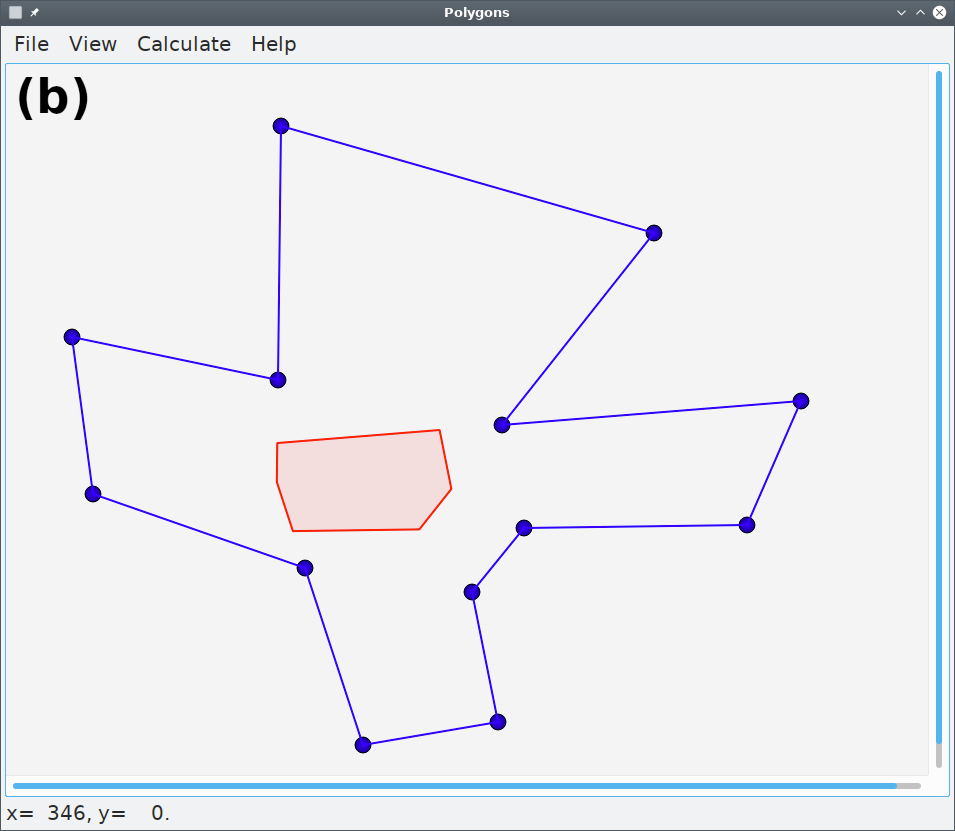
\includegraphics[width = 0.49 \textwidth]{figures/polygui_kernel}
	\caption[Polygon tool.]{Polygon tool.
		This program calculates the
		(a) convex sub-regions of a concave polygon, and
		(b) the visibility kernel (red) of a polygonal region.
		Polygon vertices can be inserted, deleted and moved using the mouse, updates
		are performed dynamically.
		\label{fig:linesgui}}
\end{figure}



\subsection{Convex hull tool}
\begin{figure}[htb]
	\centering
	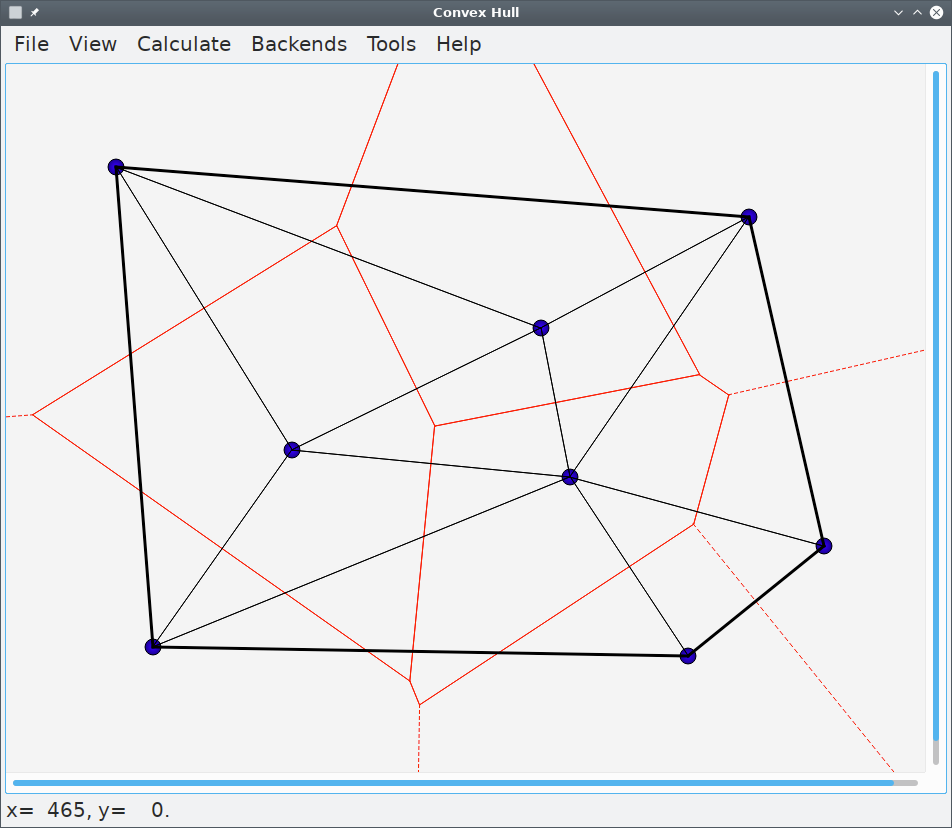
\includegraphics[width = 0.49 \textwidth]{figures/hullgui_voro}
	\hspace{0.05cm}
	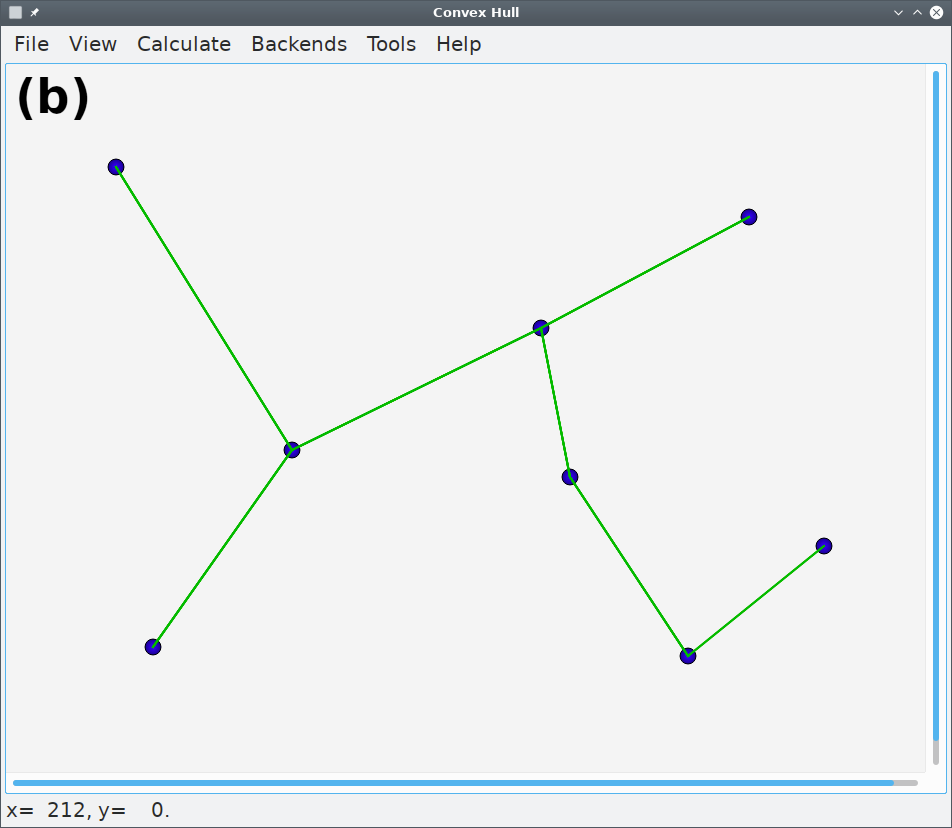
\includegraphics[width = 0.49 \textwidth]{figures/hullgui_kruskal}
	\caption[Convex hull tool.]{Convex hull tool.
		This program calculates 
		(a) the convex hull (thick black lines), the Voronoi diagram (red lines), 
			the Delaunay triangulation (thin black lines), as well as
		(b) Kruskal's minimum spanning tree (green lines)
		of a collection of vertices.
		As with the other test tools, the vertices can be inserted, deleted and moved 
		using the mouse, updates are performed dynamically.
		\label{fig:linesgui}}
\end{figure}




\section{Unit tests}
\label{sec:unit_tests}
A unit test tests if a given set of inputs to a function gives an expected set of outputs.
Testing an algorithm containing several function calls also allows to check if a set of invariants
is fulfilled during the algorithm run, meaning between function calls.
Possible checks can either be fixed input values which are testes agains known output values,
or random inputs for which the correct output is calculated independently using a different 
method than the one being tested, or even an external program.
Unit tests allow to spot an error for which they are specifically designed. Conversely, they cannot 
prove that a software is free of errors. Such a feat would be the task of software verification, 
which is very complicated, if not impossible for software systems of a certain size and complexity.

For the present software, unit tests of isolated functions and algorithms were performed using the 
C++ library \textit{Boost.Test} \cite{web_boost_test}.
In \textit{Boost.Test}, test modules are defined per unit test file, which contains one or more test cases.
These test cases can also be configured to create different instances of template functions using
different template arguments. The body of a test case contains a block of normal C++ code.
In the C++ code, conditions and invariants are tested using the 
\lstinline[language=C++]|BOOST_TEST()| macro. Each successful or non-successful evaluation
of the macro is registered by \textit{Boost.Test} and reported in a final summary.
